% This is samplepaper.tex, a sample chapter demonstrating the
% LLNCS macro package for Springer Computer Science proceedings;
% Version 2.20 of 2017/10/04
%
\documentclass[runningheads]{llncs}
%
\usepackage{graphicx}
\usepackage{xcolor}
\usepackage{url}
\usepackage{xurl} % corta las URL largas de las referencias
\usepackage[spanish,es-tabla]{babel} % "Tabla" en lugar de "Cuadro"
\usepackage{array}
\usepackage{longtable}
% titulos de longtable con el mismo formato que las tablas de llncs ("Tabla 1." en negrita)
\makeatletter
\def\LT@makecaption#1#2#3{\LT@mcol\LT@cols c{\hbox to\z@{\hss\parbox[t]\textwidth{\@makecaption{#2}{#3}}\hss}}}
\makeatother

% Used for displaying a sample figure. If possible, figure files should
% be included in EPS format.
%
% If you use the hyperref package, please uncomment the following line
% to display URLs in blue roman font according to Springer's eBook style:
% \renewcommand\UrlFont{\color{blue}\rmfamily}

\begin{document}
%
\title{carga.uy: una plataforma Jakarta EE para la gestión y fiscalización del transporte de carga}
%
\titlerunning{carga.uy: gestión y fiscalización del transporte de carga}
% If the paper title is too long for the running head, you can set
% an abbreviated paper title here
%
\author{Lucas Lazogue \and
Kevin Martínez \and
Andrés Murara \and
Eric Tift \\ \email{\{lucas.lazogue, kevin.martinez, andres.murara, eric.tift\}@fing.edu.uy}}

\authorrunning{L. Lazogue et al.}
% First names are abbreviated in the running head.
% If there are more than two authors, 'et al.' is used.

\institute{Facultad de Ingeniería - Universidad de la República \\ J. Herrera y Reissig 565, Montevideo, Uruguay \\
\url{http://www.fing.edu.uy/}}
%
\maketitle              % typeset the header of the contribution
%
\begin{abstract}
El transporte de carga por carretera sostiene buena parte de las cadenas de distribución de Uruguay, y su regulación requiere controlar la habilitación de empresas y vehículos y fiscalizar los viajes que realizan. En este artículo se presenta el diseño e implementación de carga.uy, una plataforma desarrollada sobre Jakarta EE que da soporte a la gestión del transporte de carga y a su fiscalización. La plataforma integra un frontoffice web, un backoffice, una aplicación móvil que funciona sin conectividad y nodos periféricos que simulan los sistemas de tracking y de balanzas, y autentica a los ciudadanos con Usuario gub.uy. Las posiciones de los vehículos se reciben de forma asíncrona a través de un broker de mensajería y, junto con los pesajes y los datos declarados por las empresas, alimentan la detección automática de incumplimientos. Se presentan la arquitectura de la solución, las tecnologías utilizadas y una evaluación preliminar de la ingesta de tracking y de la resiliencia ante fallas.

\sloppy
\keywords{Jakarta EE \and Mensajería asíncrona \and Observabilidad \and Computación en la Nube.}
\end{abstract}
%
%
%

\section{Introducción}

\subsection{Motivación}

Todas las actividades económicas dependen de cadenas de distribución: tanto en la llegada de materias primas a centros industriales como en la distribución de todo tipo de productos para llegar a los consumidores finales. En Uruguay a nivel interno la mayoría del transporte de dichas cadenas de distribución se realiza a través del transporte carretero. El Estado como regulador de todas las actividades también regula el Transporte de Carga a través de la Dirección Nacional de Transporte\footnote{\raggedright\url{https://www.gub.uy/ministerio-transporte-obras-publicas/institucional/estructura-del-organismo/direccion-nacional-transporte}} del Ministerio de Transporte y Obras Públicas\footnote{\raggedright\url{https://www.gub.uy/ministerio-transporte-obras-publicas/}}. Hay muchas normativas relacionadas a la regulación del transporte de carga\footnote{\raggedright\url{https://www.gub.uy/ministerio-transporte-obras-publicas/politicas-y-gestion/transporte-carga}} que se han ido actualizando con el avance de la tecnología y los avances en gobierno electrónico.

El Estado necesita contar con información sobre la actividad del transporte de carga para objetivos de recaudación, la fiscalización de la actividad y la planificación de la infraestructura necesaria a futuro. Para esto existe un registro de las empresas transportistas, que a su vez tienen que registrar y sacar permisos para sus vehículos (así como hacerle periódicamente una Inspección Técnica Vehicular). Cada vez que un vehículo realiza un viaje con carga se genera un documento llamado “Guía” que indica toda la información de la carga y el viaje a realizarse. A su vez para poder hacer seguimiento de dichos viajes se tiene que los GPS de los vehículos de carga transmiten su información de posición a un sistema central. También durante la realización de viajes los vehículos de carga pasan por balanzas que están ubicadas en los peajes de las rutas nacionales.

Toda esta operativa requiere que se esté fiscalizando tanto la habilitación de los vehículos como los viajes que realizan (por ejemplo que no excedan su capacidad de carga). Por esto, dentro del MTOP hay funcionarios que realizan tareas de administración de estos sistemas y pueden gestionar a los demás usuarios que tendrán acceso a ellos; funcionarios que realizan tareas operativas de fiscalización y autoridades que reciben informes cuantitativos agregados de la información operativa. Este sistema también brinda información agregada al público en general y brinda servicios de consulta a empresas que requieren los servicios de transporte de carga y quieren validar las autorizaciones de las empresas que contratan.

El volumen de información que maneja esta operativa no es menor: los dispositivos GPS de la flota reportan su posición de forma continua mientras los viajes están en curso. Además, las balanzas de los peajes registran pesajes en forma permanente. Cruzar esa información con los datos declarados por las empresas (capacidad de carga de cada vehículo, vigencia de permisos e ITV, origen y destino de cada Guía) es lo que permite detectar incumplimientos sin depender de un control manual exhaustivo. Actualmente, esta detección es mayormente reactiva; se busca que la plataforma la realice de forma automática y que los funcionarios se concentren en la resolución de los casos detectados.

Para colaborar en esto se propone la construcción de una plataforma que brinde soporte a todo el ciclo de la gestión de transporte de carga. Los principales objetivos son:

\begin{itemize}
    \item Posibilitar que las Empresas transportistas puedan registrarse y registrar sus vehículos.
    \item Posibilitar que los funcionarios del MTOP puedan monitorear datos de las empresas y los vehículos.
    \item Posibilitar que otras empresas (clientes) puedan validar las autorizaciones de las empresas transportistas.
    \item Brindar información gerencial a las autoridades del MTOP.
    \item Brindar información estadística al público en general.
    \item Detectar automáticamente incumplimientos a la normativa de transporte de carga y dar soporte a su tramitación.
\end{itemize}

Para cumplir con estos cometidos se apunta a que la plataforma a desarrollar se apoye en algunas soluciones existentes:

\begin{itemize}
    \item servicios ofrecidos por organismos públicos a través de la Plataforma de Interoperabilidad (PDI)\footnote{\raggedright\url{https://www.gub.uy/agencia-gobierno-electronico-sociedad-informacion-conocimiento/tematica/catalogo-plataforma-interoperabilidad}}, que brindan acceso a información de trámites, personas y empresas, entre otros;
    \item Proveedores de Identidad (Usuario Gub.uy) para realizar la autenticación.
\end{itemize}


Este trabajo se desarrolló en el marco de la edición 2026 del curso Taller de Sistemas Empresariales de la Facultad de Ingeniería de la Universidad de la República.

El resto del documento se organiza de la siguiente manera. La Sección 2 presenta los conceptos necesarios para comprender el trabajo y la Sección 3 describe el problema planteado. La Sección 4 presenta la solución propuesta, la Sección 5 su arquitectura y la Sección 6 los detalles de implementación. La Sección 7 evalúa la solución y la Sección 8 describe el desarrollo del proyecto. Por último, la Sección 9 presenta las conclusiones y el trabajo a futuro.

\section{Marco Teórico}
En esta sección se describen los conceptos necesarios para comprender la solución: servicios web, autenticación y autorización, mensajería asíncrona, bases de datos documentales y observabilidad.

\subsection{Servicios web}
Los servicios web exponen funcionalidades que otras aplicaciones pueden invocar a través de una red. Facilitan la comunicación entre aplicaciones desarrolladas sobre distintas plataformas de hardware y software \cite{OracleWebServices}.

REST es un estilo arquitectónico utilizado para diseñar API web. Se basa en una arquitectura cliente-servidor, comunicación sin estado y una interfaz uniforme. Una API REST entrega al cliente representaciones de los recursos solicitados mediante HTTP, utilizando formatos como JSON \cite{RedHatREST}.

SOAP es un protocolo que permite intercambiar mensajes entre aplicaciones desarrolladas con distintos lenguajes y plataformas. Utiliza mensajes en formato XML y puede emplear HTTP para su transmisión \cite{RedHatSOAPREST}.

\subsection{Autenticación y autorización}
La autenticación verifica la identidad de un usuario a partir de las credenciales que presenta. La autorización determina los recursos a los que puede acceder y las operaciones que puede realizar. En el control de acceso basado en roles, los permisos dependen del rol asignado al usuario dentro del sistema \cite{IBMAuth}.

OpenID Connect (OIDC) es un protocolo de autenticación basado en OAuth 2.0. Permite que una aplicación delegue la autenticación en un proveedor de identidad y reciba información sobre el usuario autenticado mediante un token de identidad \cite{MDNFederatedIdentity}.

LDAP (\textit{Lightweight Directory Access Protocol}) es un protocolo de acceso a servicios de directorio. La información del directorio se organiza en entradas con una estructura jerárquica. El protocolo permite buscar, agregar, modificar y eliminar estas entradas \cite{IBMLDAP}.

\subsection{Mensajería asíncrona}
En la mensajería asíncrona, las aplicaciones se comunican a través de un intermediario, llamado \textit{broker}: el emisor deposita un mensaje en una cola y el receptor lo consume cuando está disponible. Si el receptor no está disponible, los mensajes esperan en la cola sin perderse, y si varias instancias consumen la misma cola, cada mensaje se entrega a una sola de ellas \cite{Hohpe2003}. Jakarta Messaging (JMS) es la especificación de Jakarta EE para este modelo \cite{JakartaMessaging}.

\subsection{Bases de datos documentales}
Las bases de datos documentales son bases NoSQL que almacenan la información como documentos con estructura similar a JSON, agrupados en colecciones y sin un esquema fijo de tablas \cite{MongoDBDocuments}. Se adaptan a grandes volúmenes de datos que se agregan en forma continua y se consultan por pocos criterios.

\subsection{Observabilidad}
La observabilidad es la capacidad de entender el estado interno de un sistema a partir de los logs, las métricas y las trazas que emite \cite{OTelObservability}. Una traza distribuida registra el recorrido de una operación por varios componentes; cada tramo, llamado \textit{span}, indica qué componente lo ejecutó y cuánto duró. Para unir los spans de distintos componentes, el contexto de la traza viaja con cada solicitud, por ejemplo en el encabezado \texttt{traceparent} de W3C Trace Context \cite{W3CTraceContext}. OpenTelemetry es un estándar abierto que define las API, los SDK y el protocolo (OTLP) para generar y exportar esta información \cite{OTelObservability}.

\section{Descripción del Problema}

El problema planteado consiste en el diseño y construcción de carga.uy, una plataforma para gestionar el transporte de carga y apoyar su fiscalización en Uruguay.

Las funcionalidades para las empresas transportistas se ofrecen mediante un frontoffice web del componente central. El responsable de una empresa puede gestionar su perfil, sus vehículos, permisos, inspecciones, guías de viaje e infracciones. La aplicación móvil permite que los choferes consulten el viaje asignado y registren el comienzo, la finalización, cargas o descargas parciales e incidentes, incluso cuando no disponen de conectividad.

Los funcionarios acceden a un frontoffice web para gestionar empresas, fiscalizar permisos y vehículos, monitorear viajes y resolver casos de fiscalización. Las autoridades utilizan un backoffice web para consultar reportes e indicadores. Los administradores utilizan el mismo backoffice para gestionar usuarios, roles, nodos periféricos y parámetros de las reglas de fiscalización.

Los nodos de balanzas suministran los pesajes registrados en los peajes y los nodos de tracking reportan periódicamente la posición de los vehículos. La Plataforma de Interoperabilidad permite consultar datos de organismos públicos, mientras que Usuario gub.uy proporciona la autenticación de ciudadanos y funcionarios.

La plataforma debe implementarse sobre Jakarta EE, con el componente central desplegado en la nube y los nodos periféricos en una plataforma distinta. Además de los requerimientos obligatorios, se plantean doce requerimientos opcionales, de los que se eligieron cuatro: LDAP como mecanismo de autenticación interna del backoffice, el despliegue del componente central en un orquestador de contenedores con escalado horizontal, una base de datos NoSQL para los eventos de posición y una base de datos con soporte geoespacial para las rutas y el cálculo de desvíos.

\section{Solución Propuesta}

\subsection{Descripción General}
La solución desarrollada se organiza en un componente central, una aplicación móvil y nodos periféricos de balanzas y tracking. El componente central cuenta con un frontoffice web con una sección pública y áreas de acceso autenticado para empresas transportistas y funcionarios, y un backoffice para autoridades y administradores. Estas interfaces ofrecen funcionalidades de gestión de empresas, vehículos y viajes, fiscalización, consulta de reportes y administración de usuarios. La Figura \ref{fig:descripcion-general} presenta una vista general de la plataforma, sus usuarios y los sistemas externos con los que se integra. A continuación, se describen los principales aspectos de la solución.

\begin{figure}
\centering
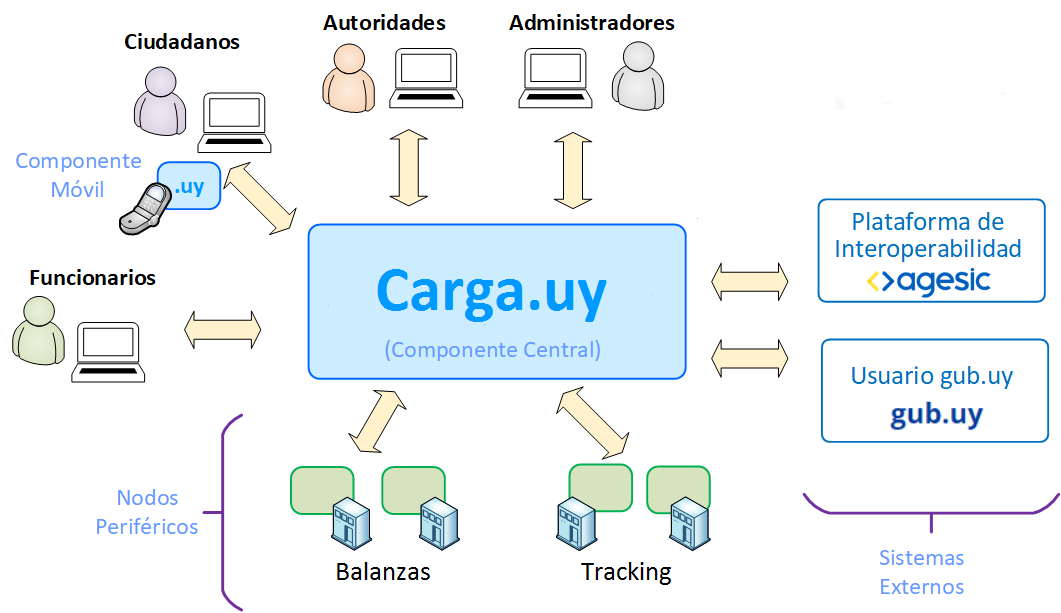
\includegraphics[width=\textwidth]{figuras/descripcion-general.png}
\caption{Descripción General de la Solución} \label{fig:descripcion-general}
\end{figure}


\subsection{Gestión de empresas, vehículos y viajes}
El frontoffice permite a los responsables gestionar la información de su empresa, sus vehículos y las guías de carga. A partir de una guía se asigna un viaje a un vehículo y un chofer de la empresa, comprobando la vigencia de sus habilitaciones y del vínculo del chofer. Los permisos ingresados por el responsable quedan pendientes de revisión por un funcionario, quien puede aprobarlos indicando su período de validez o rechazarlos dejando un motivo. El acceso a estas operaciones se controla en la capa de servicios según el rol del usuario y su relación con la empresa.

\subsection{Autenticación y acceso}
El frontoffice y la aplicación móvil utilizan Usuario gub.uy mediante OpenID Connect. El componente central recibe el código de autorización y lo intercambia con gub.uy para obtener la identidad del usuario. A partir de su cédula busca el registro correspondiente y, si es un ciudadano que ingresa por primera vez, lo crea. Los roles se obtienen de la información registrada en el componente central.

El central genera un JWT propio firmado, cuyos claims incluyen el identificador del usuario, la cédula, los roles, el correo cuando está disponible, el emisor, el tipo de token y las fechas de emisión y vencimiento. En el frontoffice se guarda en una cookie HttpOnly que acompaña las solicitudes. El central verifica la firma, la vigencia, el emisor y el tipo del token para identificar al usuario y sus roles.

La aplicación móvil realiza el ingreso desde el navegador, pero no comparte automáticamente sus cookies. Para obtener su token utiliza un intercambio con PKCE: genera y guarda un valor aleatorio, llamado code\_verifier, calcula su SHA-256 para obtener el code\_challenge y lo envía al endpoint de autenticación del central mediante el navegador. Tras completar el ingreso con gub.uy, el central devuelve a la aplicación un código temporal asociado al challenge. La aplicación envía ese código junto con el verifier al central, que verifica la validez del código y calcula nuevamente el SHA-256 del verifier para comprobar que coincida con el challenge antes de entregar el JWT.

Para las autoridades y los administradores, el backoffice utiliza un directorio LDAP, cuyos grupos determinan los roles de acceso. La administración de las cuentas del backoffice se realiza desde la propia aplicación.

\subsection{Aplicación móvil}
La aplicación móvil está destinada a los choferes. Tras el ingreso, descarga los viajes asignados y en curso del chofer junto con su Guía y los guarda en una base de datos local, de modo que puede consultarlos y operar sin conectividad. Desde el detalle de un viaje, el chofer registra el inicio y el fin, las cargas y descargas parciales con sus kilos y los incidentes con una descripción. La aplicación solo ofrece las acciones válidas para el estado del viaje y valida los datos con las mismas reglas que el componente central. Para que pueda seguir trabajando sin conexión, la sesión se mantiene con un token de renovación ligado a una clave del dispositivo guardada en el Android Keystore, por lo que una copia de ese token no sirve en otro equipo.

Cada evento se guarda primero en el dispositivo, con un identificador UUID generado localmente y la hora en que ocurrió, y luego se envía al central en segundo plano. El envío es una tarea que espera a que haya conexión, se ejecuta aunque la aplicación esté cerrada y, si falla, se reintenta con esperas crecientes. El central procesa cada evento en una transacción propia, de modo que uno inválido no afecta a los demás, y responde con un resultado por evento: aplicado, duplicado, en conflicto o rechazado. Como el identificador lo genera el dispositivo, un evento reenviado tras perderse la respuesta se reconoce como duplicado y no se aplica dos veces. El estado del viaje lo decide el central: un evento sobre un viaje que ya no pertenece al chofer se registra como conflicto, y uno incompatible con el estado del viaje o fuera de su horario, como rechazado. En ambos casos el evento se conserva y el chofer ve el motivo en la aplicación. Los eventos se aplican según la hora en que ocurrieron y no la de llegada, por lo que un inicio registrado sin conectividad fija la hora de inicio real y permite asociar al viaje las posiciones de tracking recibidas antes.

\subsection{Integración con balanzas}
La integración con balanzas se realiza mediante nodos periféricos que simulan los sistemas de los operadores de peajes. Cada nodo mantiene la información de sus peajes, balanzas y pesajes, y permite consultar las lecturas de un vehículo para una fecha determinada. Para obtener los pesajes de un viaje, el componente central consulta en paralelo los nodos habilitados y selecciona las lecturas correspondientes al horario del viaje. Cada pesaje se identifica mediante el nodo, la balanza y el identificador del registro original, para evitar duplicados al repetir las consultas. Si falla la consulta a un nodo, el central devuelve los resultados obtenidos de los demás e identifica los nodos que no pudieron consultarse.

\subsection{Generación asíncrona de reportes}
La exportación de reportes se realiza en segundo plano, de modo que la autoridad pueda solicitar un informe y volver más adelante para descargarlo. Al solicitarlo, se guardan los filtros seleccionados, el formato y el usuario solicitante, y el informe queda en estado pendiente. La solicitud se envía a una cola para su procesamiento. Cuando finaliza la generación, el archivo queda disponible en CSV o PDF en la sección de exportaciones del usuario. Si la generación falla, se registra ese estado y la autoridad puede realizar una nueva solicitud. Cada autoridad puede consultar y descargar únicamente sus propias exportaciones.


\subsection{Ingesta de eventos de tracking}
Los nodos de tracking no invocan al componente central: publican las posiciones en una cola del broker de mensajería, por TLS y con un usuario propio por nodo que solo puede publicar en esa cola. Si el central no está disponible o recibe más posiciones de las que puede procesar, estas esperan en la cola, y ante una saturación el broker las guarda en disco en lugar de descartarlas.

En el central, un Message-Driven Bean consume las posiciones, descarta las de nodos no registrados o deshabilitados y almacena el resto en una base de datos documental. Un índice único por nodo e identificador de evento evita guardar dos veces una posición reenviada. Cada posición se asocia al viaje que el vehículo tenía en curso cuando se generó, no cuando llegó: así, una posición demorada por falta de cobertura queda en su viaje. Si el chofer inicia el viaje sin conectividad, las posiciones previas al aviso de inicio se reasocian al viaje cuando este llega. Esto evita detectar viajes sin Guía que no lo son. Confirmada la transacción, el central dispara en segundo plano la evaluación de las reglas de fiscalización.

Si el procesamiento falla, por ejemplo porque la base de datos no responde, el broker reentrega la posición con una espera creciente, de uno a sesenta segundos, durante unos catorce minutos; si todos los intentos fallan, la posición pasa a una cola de mensajes muertos, desde la que puede reprocesarse. Varias instancias del central pueden consumir la misma cola para escalar la ingesta.

\subsection{Fiscalización automática}
\textcolor{red}{[Completar: reglas evaluadas, disparo desde la ingesta y desde el fin del viaje, deduplicación de casos, reevaluación ante balanzas no disponibles y ciclo del caso.]}

\subsection{Gestión de nodos periféricos}
El administrador registra cada nodo periférico desde el backoffice con su identificador, tipo y punto de acceso; para los nodos de balanzas, también la clave con la que el central se autentica, que se guarda cifrada. Todo nodo nuevo queda deshabilitado hasta que el administrador lo habilita, y vuelve a deshabilitarse si cambia su punto de acceso, porque un nodo mal configurado no produce errores visibles: el central aceptaría posiciones de una fuente no verificada o consultaría una dirección incorrecta.

\subsection{Observabilidad}
La plataforma utiliza OpenTelemetry. WildFly instrumenta automáticamente los servicios REST y las llamadas a otros sistemas; donde el contexto no se propaga solo, se pasa en forma explícita: en las propiedades de cada mensaje JMS, en la evaluación de reglas en segundo plano y en las consultas en paralelo a los nodos de balanzas. La aplicación móvil también envía el contexto en cada solicitud. Así, el fin de un viaje registrado desde el celular puede seguirse en una sola traza que incluye la sincronización, la evaluación de las reglas y la consulta a cada nodo de balanzas. Los logs incluyen el identificador de la traza. La telemetría se envía por OTLP a una plataforma con Prometheus, Tempo, Loki y Grafana, donde un tablero reúne las métricas de la ingesta, la cola, los nodos, la API, las integraciones y los health checks.

\section{Arquitectura del Sistema}
El componente central se organiza en capas de presentación, servicios de negocio, persistencia e integración. La presentación comprende los frontoffices, el backoffice y la API REST utilizada por los clientes. Los servicios de negocio concentran las validaciones y los controles de acceso a las operaciones, mientras que la persistencia permite almacenar y consultar la información del sistema. La integración con Usuario gub.uy, la PDI y los nodos de balanzas se realiza mediante adaptadores que separan la comunicación con estos sistemas de la lógica de negocio. La Figura \ref{fig:vista-logica} presenta la arquitectura general del sistema.

\begin{figure}
\centering
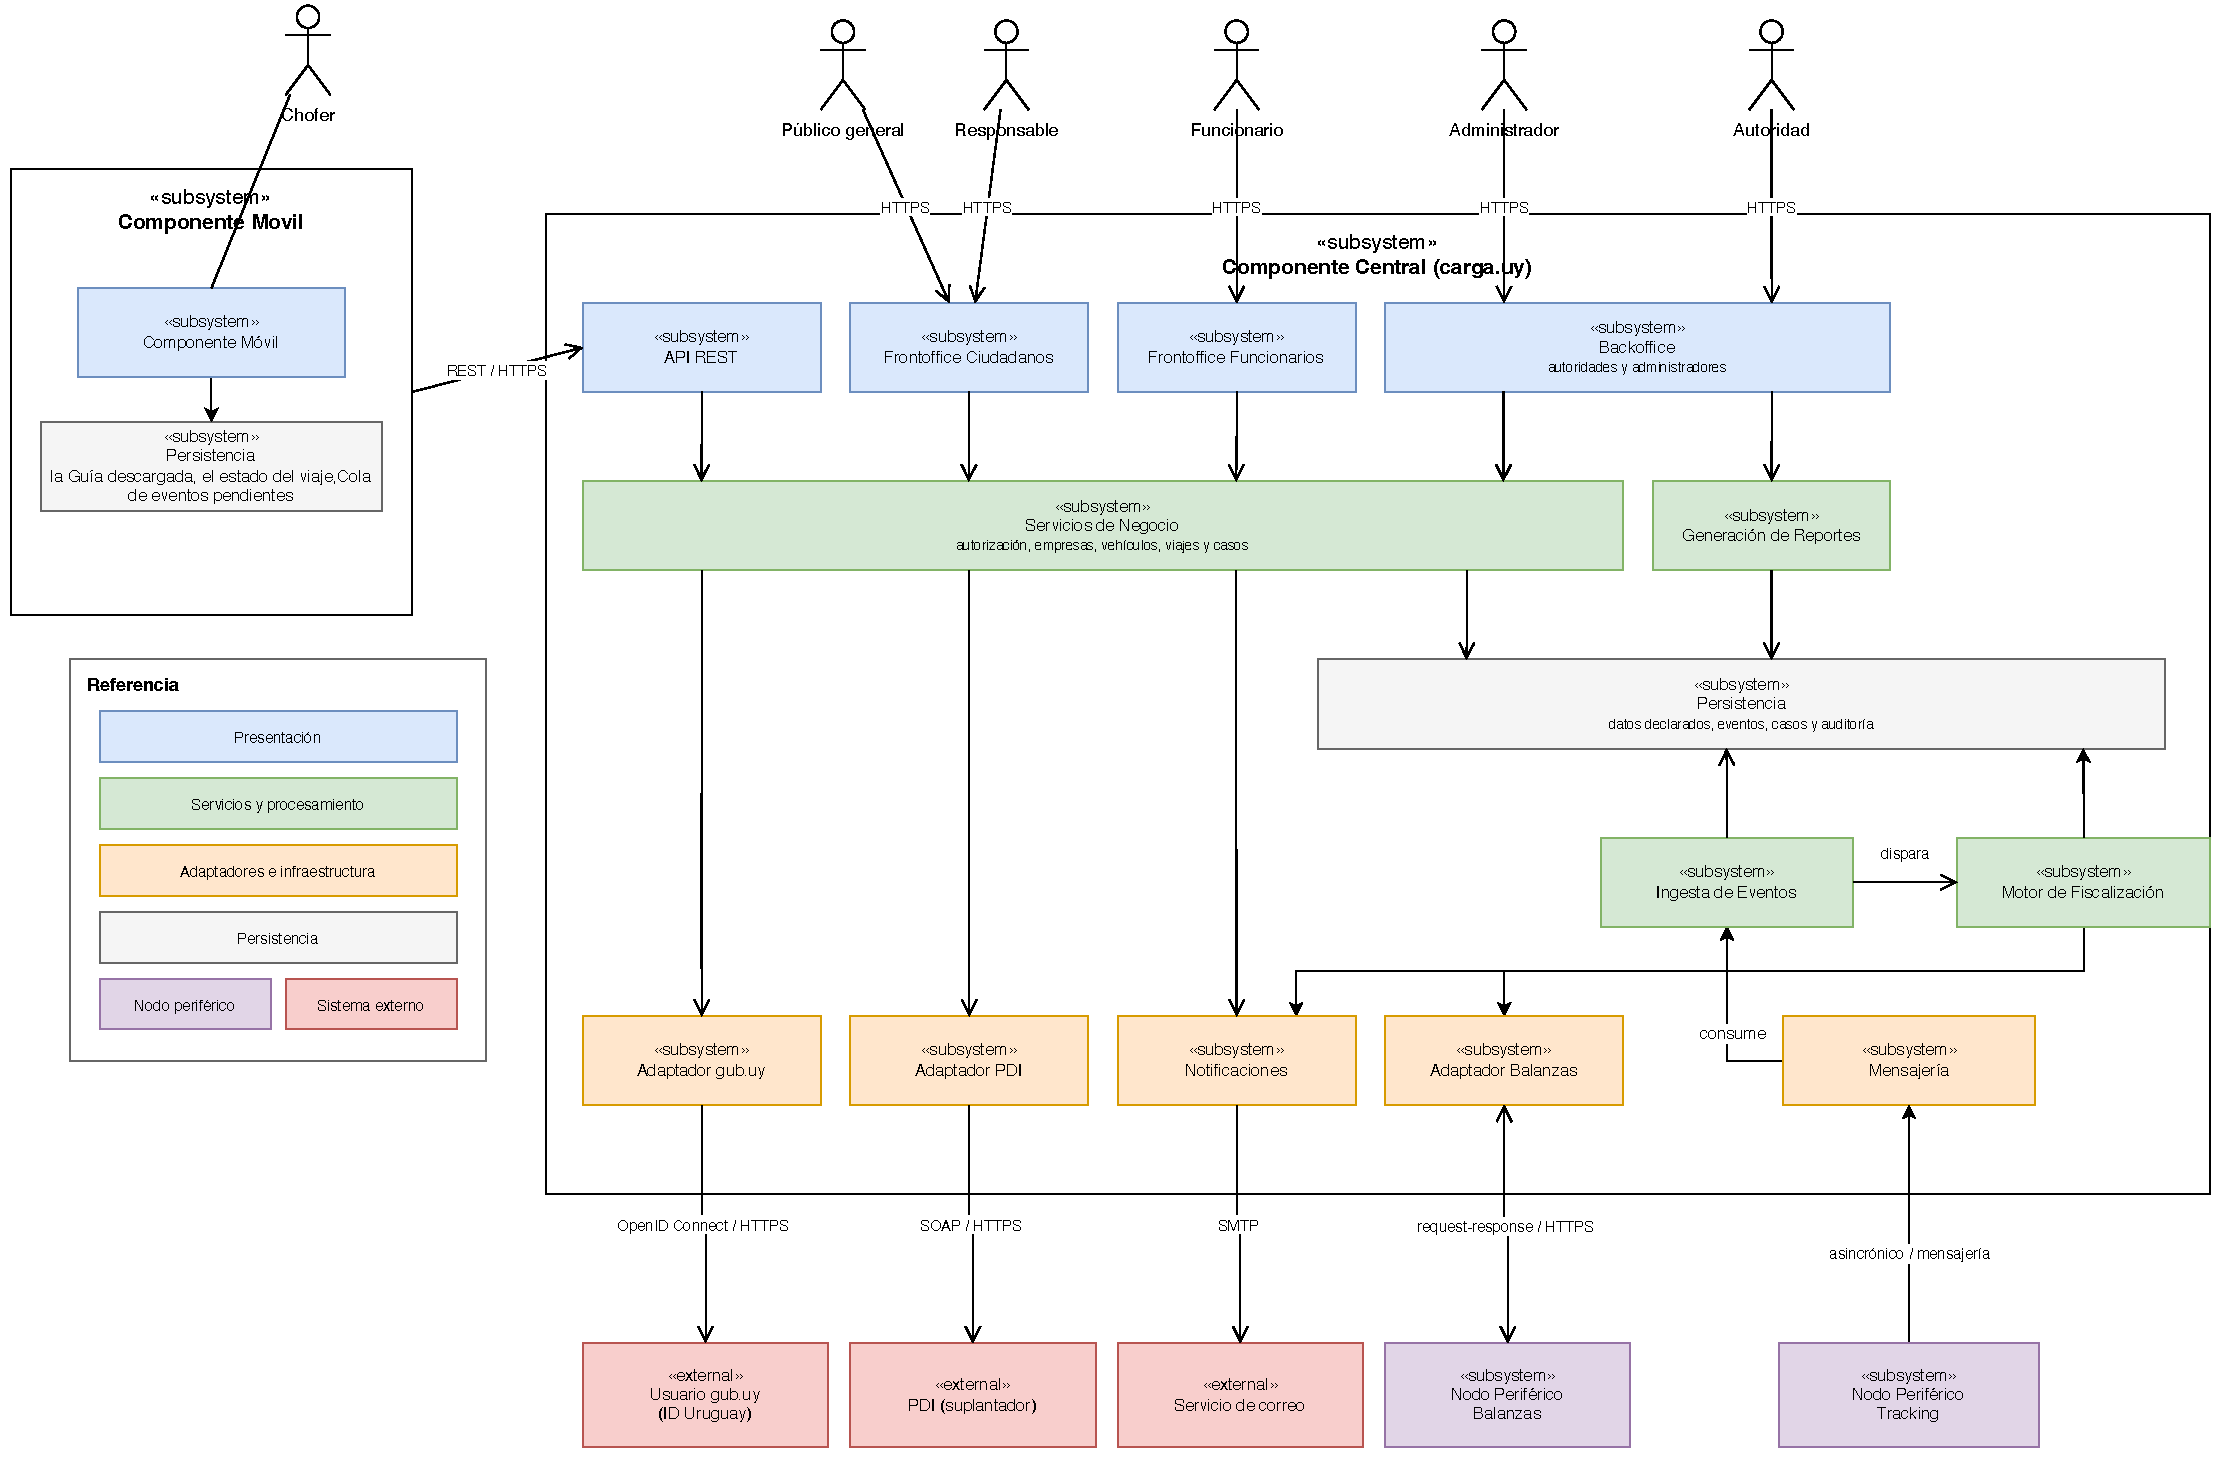
\includegraphics[width=\textwidth]{figuras/vista-logica.pdf}
\caption{Arquitectura general del sistema}
\label{fig:vista-logica}
\end{figure}

La recepción de las posiciones de tracking sigue un camino asíncrono: los nodos de tracking publican en un broker de mensajería que se ejecuta separado del servidor de aplicaciones, y el central las consume y las almacena en una base de datos documental, separada de la base relacional.

\section{Detalles de Implementación}

\subsection{Productos y Herramientas}
El componente central utiliza Jakarta EE sobre WildFly, aprovechando los servicios que proporciona el servidor para ejecutar la aplicación. La lógica de negocio se implementa mediante EJB, la persistencia mediante JPA y los servicios REST mediante JAX-RS. WildFly gestiona las transacciones y las conexiones a la base de datos. El acceso a las operaciones se restringe mediante la anotación @RolesAllowed de Jakarta EE, que indica los roles permitidos y cuya comprobación realiza el servidor.

Para almacenar los datos de empresas, vehículos, viajes y demás entidades del componente central se utilizó PostgreSQL, una base de datos relacional. El acceso se realiza mediante Jakarta Persistence (JPA), con Hibernate como implementación proporcionada por WildFly. Esto permite representar las tablas y sus relaciones mediante entidades Java. La conexión se configura como un recurso del servidor, integrando las operaciones de persistencia con las transacciones de los servicios de negocio.

Para la comunicación asíncrona se utiliza Jakarta Messaging (JMS), integrado con un broker Apache ActiveMQ Artemis que se ejecuta en un contenedor separado. Los mensajes se envían a colas y se procesan mediante Message-Driven Beans (MDB), componentes ejecutados por WildFly al recibir los mensajes. Esta integración se utiliza para la recepción de eventos de tracking y la generación de reportes, permitiendo separar el envío de las solicitudes de su procesamiento.

Para las interfaces del backoffice se utilizó Jakarta Faces, una tecnología de Jakarta EE para construir interfaces web mediante componentes, cuya implementación es proporcionada por WildFly. Sobre esta base se incorporó PrimeFaces, una biblioteca adicional de componentes para Jakarta Faces, que permitió construir formularios, tablas paginadas y diálogos.

Para el directorio de usuarios del backoffice se utilizó 389 Directory Server. Se eligió por contar con una imagen de contenedor publicada por el propio proyecto y por gestionar el almacenamiento de contraseñas con \textit{salt}, sin implementar ese mecanismo en la aplicación. También permite configurar el bloqueo por intentos de ingreso fallidos. Como trabajo adicional, fue necesario configurar la creación de la estructura del directorio y la carga inicial de los datos.

Para las posiciones de tracking se utilizó MongoDB, una base de datos documental. Son el mayor volumen de datos del sistema, se agregan en forma continua y se consultan por vehículo o por viaje; separarlas de PostgreSQL evita que ese volumen afecte a las operaciones transaccionales.

Para la observabilidad se utilizaron los subsistemas de OpenTelemetry y Micrometer de WildFly, el SDK de OpenTelemetry en el nodo de tracking y en la aplicación móvil, y la imagen \texttt{grafana/otel-lgtm}, que reúne el colector, Prometheus, Tempo, Loki y Grafana en un solo contenedor, pensada para desarrollo y pruebas. El entorno completo, con dos nodos de tracking y dos de balanzas, se levanta con un único comando mediante Docker Compose; el nodo de tracking incluye un generador de carga para las pruebas de performance.

La Tabla~\ref{tab:evaluacion-productos-herramientas} resume la evaluación de los principales productos utilizados.

\begin{table}
\caption{Evaluación de Productos y Herramientas.}\label{tab:evaluacion-productos-herramientas}
\begin{tabular}{|>{\raggedright\arraybackslash}p{2.5cm}|>{\raggedright\arraybackslash}p{3cm}|>{\raggedright\arraybackslash}p{3cm}|>{\raggedright\arraybackslash}p{3cm}|}
\hline
    Producto &  Puntos Fuertes & Puntos Débiles & Evaluación General\\
\hline
    ActiveMQ Artemis & Integrado con WildFly; reentregas, cola de mensajes muertos y paginado a disco. & Protocolo propio sobre TCP, difícil de exponer en plataformas que solo publican HTTP. & Adecuado: sin pérdida de posiciones con el central detenido. \\
\hline
    MongoDB & Escritura rápida; índice único para descartar duplicados. & Sin transacciones compartidas con PostgreSQL. & Adecuado para las posiciones. \\
\hline
    OpenTelemetry y Grafana & Estándar abierto; instrumentación automática en WildFly. & La propagación por mensajería y en procesos asíncronos requirió código propio. & Permitió diagnosticar fallas de punta a punta. \\
\hline
    \textcolor{red}{[Productos del resto de los lotes]} & & & \\
\hline
\end{tabular}
\end{table}


\subsection{Problemas Encontrados}

\textbf{Trazas interrumpidas.} La instrumentación automática no propaga el contexto de la traza a los hilos de un ejecutor, a los métodos asíncronos de los EJB ni a los observadores que se ejecutan tras confirmar una transacción, por lo que esos pasos aparecían como trazas independientes. Se resolvió pasando el contexto en forma explícita.

\textbf{Caída de la base de datos.} Al detener PostgreSQL unos segundos, el broker agotaba los reintentos inmediatos y las posiciones terminaban en la cola de mensajes muertos; al volver la base, el central conservaba conexiones inválidas. Se configuraron reentregas con espera creciente y la validación de las conexiones del pool.

\textcolor{red}{[Despliegue: Elastic Cloud no estuvo disponible y el componente central se desplegó en OpenShift. Completar.]}

\section{Evaluación de la Solución}
\subsection{Puntos fuertes y débiles}
Entre los puntos fuertes de la solución se destacan la separación entre la recepción de los eventos y su procesamiento, que permite tolerar la indisponibilidad del componente central y de los nodos periféricos sin perder información; el control de acceso aplicado en la capa de servicios y no solo en las interfaces; la posibilidad de seguir cada operación de punta a punta mediante trazas distribuidas; y un entorno de desarrollo completo que se levanta con un solo comando.

Entre los puntos débiles, al momento de esta entrega quedan pendientes la regla de desvío de ruta, que requiere calcular el recorrido esperado con soporte geoespacial; la consulta a la PDI en el primer ingreso; la asignación de choferes a una empresa; el filtro por ubicación de los reportes; la validación de viajes solapados de un mismo vehículo; y la notificación de los casos por correo. Además, la performance se evaluó solo en forma preliminar.

\subsection{Volumen de tracking y performance de la ingesta}
El volumen objetivo se estimó a partir de los 17.869 vehículos con motor registrados para el transporte profesional de carga \cite{BID2022}, de las 2.050 horas de trabajo por año que el MTOP considera para un camión pesado \cite{INALOG2021} y de un factor de hora pico de entre el 10~\% y el 16~\% del tránsito diario \cite{PennDOT2021}: en la hora pico habría entre 10.000 y 16.000 vehículos en viaje. Se tomaron 15.000 vehículos que reportan una posición cada 30 segundos, una frecuencia que fija la plataforma: 500 posiciones por segundo, con picos del triple.

Una prueba preliminar, con todos los componentes y el generador de carga en una misma computadora de 8 núcleos, dio los resultados de la Tabla~\ref{tab:prueba-preliminar}. Hasta 250 posiciones por segundo la cola se mantiene acotada; con 500, el central procesa en promedio lo que llega, pero la computadora se satura. El procesamiento de cada posición no supera los 8~ms en el percentil 95, por lo que el cuello de botella, identificado con las métricas de la plataforma de observabilidad, es la CPU compartida y no la ingesta. Queda pendiente repetir la prueba con el generador separado y el central en la nube, medir el frontoffice bajo carga y verificar el escalado horizontal.

\begin{table}
\caption{Prueba preliminar de la ingesta de tracking.}\label{tab:prueba-preliminar}
\centering
\begin{tabular}{|r|r|r|r|}
\hline
Objetivo (pos/s) & Procesadas (pos/s) & Cola máxima & Procesamiento p95 \\
\hline
100 & 88 & 1.002 & 38 ms \\
\hline
250 & 279 & 2.192 & 8,4 ms \\
\hline
500 & 521 & 9.932 & 7,7 ms \\
\hline
\end{tabular}
\end{table}

\subsection{Resiliencia ante fallas}
Con el componente central detenido, el nodo de tracking siguió publicando y las posiciones esperaron en la cola; al reiniciarlo, se procesaron todas. Con PostgreSQL detenido durante un minuto, el central se recuperó sin intervención y ninguna posición llegó a la cola de mensajes muertos. Al detener un nodo de balanzas, el caso de exceso de carga se registró con los pesajes del otro nodo, y el pesaje faltante se agregó al mismo caso cuando el nodo volvió.

\section{Desarrollo del Proyecto}
El trabajo se dividió en cuatro lotes, uno por integrante: la operativa de empresas, el backoffice y la integración con balanzas; la aplicación móvil, la identidad y el despliegue; la ingesta de eventos, los nodos periféricos, la performance y la observabilidad; y la fiscalización automática. Las decisiones de arquitectura que afectaban a más de un lote se discutieron en conjunto y se registraron en el documento de arquitectura.

El código se gestionó en un repositorio Git. Cada cambio se desarrolló en una rama propia y se integró a la rama principal mediante un pull request; entre el 6 de octubre y el 2 de noviembre se integraron 81. Un pipeline de integración continua compila el componente central, ejecuta las pruebas automatizadas y valida el frontoffice y la aplicación móvil en cada cambio, y desde una rama de release se despliegan automáticamente el frontoffice y el componente central. El documento de arquitectura se mantuvo en LaTeX en el mismo repositorio, lo que permitió revisar sus cambios con el mismo proceso que el código.

El seguimiento se realizó mediante monitoreos semanales con el docente. Las entregas intermedias se corrieron una semana respecto de las fechas previstas en la letra. La principal desviación fue el despliegue: la plataforma Elastic Cloud prevista para el componente central no estuvo disponible, por lo que se buscó una alternativa.

\textcolor{red}{[Completar: porcentaje de tiempo dedicado a cada tarea y comparación con el cronograma inicial.]}

\section{Conclusiones y Trabajo a Futuro}
\textcolor{red}{[Borrador: revisar entre todos.]}

Se diseñó e implementó una plataforma que da soporte a la gestión del transporte de carga y a su fiscalización, integrando un frontoffice, un backoffice, una aplicación móvil y nodos periféricos de tracking y de balanzas. Los servicios que provee el servidor de aplicaciones (transacciones, seguridad declarativa, mensajería y ejecución asíncrona) permitieron concentrar el desarrollo en la lógica del negocio. La comunicación asíncrona con los nodos de tracking y la idempotencia en la ingesta y en la sincronización de la aplicación móvil permiten tolerar fallas sin perder información, lo que se comprobó en las pruebas de resiliencia. La observabilidad resultó útil también durante el desarrollo, para diagnosticar fallas que de otro modo habrían sido difíciles de reproducir.

Como trabajo a futuro queda completar la regla de desvío de ruta a partir del recorrido esperado calculado con soporte geoespacial, la consulta a la PDI, el filtro por ubicación de los reportes y la validación de viajes solapados; desplegar los nodos periféricos en una plataforma distinta a la del componente central; y repetir la prueba de performance sobre el despliegue en la nube, con el generador de carga separado y varias instancias del componente central.

\bibliographystyle{plain}
\bibliography{references}

\end{document}
